\chapter{Elektrische Netzwerke}
\label{v:13}

In diesem Versuch lernen Sie grundlegende Schaltungen kennen, die die Bestimmung eines unbekannten ohmschen Widerstandes durch Strom- und Spannungsmessungen erlauben. 

%------------------------------------------------
\section{Stichworte}
%------------------------------------------------

Spannung und Strom; Spannungs- und Strommessung; Widerstand, Ohm'sches Gesetz; Kirchhoff'sche Gesetze; Wheatstone'sche Br"uckenschaltung; Innenwiderstand; Spannungsteilerschaltung.
%
%------------------------------------------------
\section{Literatur}
%------------------------------------------------

Gehrtsen, Kapitel 6.1.2, 6.3.1 - 6.3.4
%
%------------------------------------------------
\section{Anwendungsbeispiele}
%------------------------------------------------

Strom- und Spannungsmessung, Aufbau aller elektrischen Netzwerke

%------------------------------------------------
\section{Theoretischer Hintergrund}
%------------------------------------------------

\subsection{Spannung, Strom und Widerstand}

Die elektrische \textit{Spannung} ist die Differenz der Coulombpotenziale an zwei Orten, zum Beispiel zwei Punkten in einem elektrischen Schaltkreis:
\begin{equation}
	U = \Phi_A - \Phi_B
\end{equation}
Wie man an dieser Definition sieht, bezieht sich die Angabe einer Spannung immer auf ein Referenzpotenzial, welches entweder explizit angegeben wird (''Spannung zwischen Punkten A und B'') oder impliziert wird (typischerweise die sogenannte ''Erde''). Daher kann eine Spannung \textit{positiv} oder \textit{negativ} sein, je nachdem ob das Potenzial am beschriebenen Punkt höher oder niedriger als das Referenzpotenzial ist. Bei einer Spanungsquelle in einem elektrischen Schaltkreis nennt man den Anschluß mit dem höheren Potenzial den \textit{Pluspol} und den mit dem niegrigeren Potenzial den \textit{Minuspol}. Bei den Schaltsymbolen in den nachfolgenden Schaltplänen bezeichnet der längere Strich an der Spannungsquelle den Pluspol.\\
Diese Potenzialdifferenz erzeugt ein elektrisches Feld ($\vec{E} = -\mathrm{grad}\Phi$), welches auf geladene Teilchen (zum Beispiel Elektronen) eine \textit{Coulombkraft} in Richtung der Feldlinien ausübt und diese damit beschleunigt. Negativ geladene Elektronen werden dabei auf den Pluspol zu beschleunigt. Die resultierende \textit{Drift} der Ladungsträger, zum Beispiel in einem Draht, nennt man dann \textit{Strom}:
\begin{equation}
	I = \frac{dQ}{dt}
\end{equation}
Die \textit{technische Stromrichtung} ist so definiert, dass Strom vom Pluspol einer Spannungsquelle zum Minuspol fließt (also entgegen der Driftrichtung von Elektronen). In den nachfolgenden Schaltplänen ist teilweise die technische Stromrichtung durch Pfeile gekennzeichnet.\\

\noindent
Die Einheiten von Spannung, $[U]~=~1~V$, und von Strom, $[I]~=~1~A$, das Volt und das Ampere, sind SI Einheiten. \\

\noindent
Der ohmsche Widerstand eines Leiters ist definiert durch das Ohm'sche Gesetz
\begin{equation}
R:=\frac{U}{I}\, ,
\end{equation}
seine Einheit $[R]~=~1$~\Ohm\, ist das \textit{Ohm}.

\subsection{Einfache Netzwerke}

Elektrische Netzwerke bestehen aus elektrischen Bauteilen, welche miteinander verbunden werden. In diesem Versuch wollen wir uns mit dem einfachsten passiven Bauteil beschäftigen: dem rein ohmschen Widerstand.\\
Netzwerke sind aus \textit{Knoten} und \textit{Maschen} aufgebaut. Aufbauend auf der Erhaltung der elektrischen Ladung ($\frac{dQ}{dt} = 0$) kann man das Verhalten von Strom und Spannung durch die \textit{Kirchhoffschen Gesetze} beschreiben:\\

\noindent
1. Kirchhoffsches Gesetz (Knotenregel): \\
	Die Summe aller Ströme, die in eine Knoten hinein bzw. aus einem Knoten herausfließen, ist null.
 \begin{equation}
  \sum^n_{k=1}{I_k} = 0 \; .
  \label{eq:Kirchhoff1}
 \end{equation}
%
2. Kirchhoffsches Gesetz (Maschenregel): \\
	Die Summe aller Spannungen in einer Masche ist null.
\begin{equation}
 \sum^n_{k=1}{U_k} = 0 \; .
 \label{eq:Kirchoff2}
\end{equation}

\noindent
Die Kirchhoffschen Gesetze können benutzt werden, um den Strom durch ein Bauteil und die über ihm abfallende Spannung zu beschreiben. Ein Beispiel ist die Berechnung des Gesamtwiderstandes einer Parallel- oder Serienschaltung von Widerständen.
%
\subsection{Parallelschaltung}

\begin{minipage}{0.35\textwidth}
 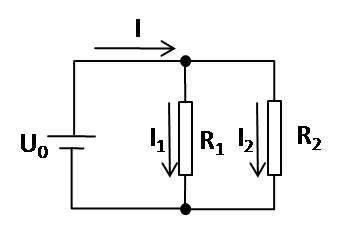
\includegraphics[width=1.00\textwidth]{Versuch_13-14/Abbildungen/Parallel.jpg}
 \label{fig:Parallel}
\end{minipage}
%
\begin{minipage}{0.6\textwidth}
Aus der Knotenregel folgt: \hfill $I = I_1 + I_2\, .$\\
Mit dem Ohm'schen Gesetz folgt: \hfill $\frac{U_0}{R_{ges}} = \frac{U_0}{R_1} + \frac{U_0}{R_2}\, .$\\
Den Gesamtwiderstand der Parallelschaltung von Widerständen kann man also schreiben als: 
\begin{equation}
\frac{1}{R_{ges}} = \frac{1}{R_1} + \frac{1}{R_2} = \sum_i{\frac{1}{R_i}} \, .
\end{equation}
\end{minipage}
%
\subsection{Serienschaltung}

\begin{minipage}{0.35\textwidth}
 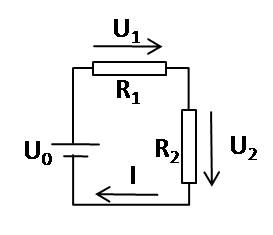
\includegraphics[width=1.00\textwidth]{Versuch_13-14/Abbildungen/Seriell.jpg}
 \label{fig:Seriell}
\end{minipage}
%
\begin{minipage}{0.6\textwidth}
Aus der Maschenregel folgt: \hfill $U_0 = U_1 + U_2\, .$\\
Mit dem Ohm'schen Gesetz folgt: \hfill $I R_{ges} = I R_1 + I R_2\, .$\\
Den Gesamtwiderstand der Serienschaltung von Widerständen kann man also schreiben als: 
\begin{equation}
R_{ges} = R_1 + R_2 = \sum_i{R_i} \, .
\end{equation}
\end{minipage}
%
\subsection{Der (unbelastete) Spannungsteiler}

In Schaltung \ref{fig:Seriell} kann man die Spannung $U_2$, die über den Widerstand $R_2$ abfällt auch als Eingangsspannung für eine daran anschliessende Schaltung benutzen. Schaltung \ref{fig:Seriell} bezeichnet man in diesem Fall als \textit{Spannungsteiler}. Die Spannung $U_2$ wird dann durch die \textit{Spannungsteilerformel} gegeben, die wir kurz herleiten wollen:\\
Fließt ein Strom $I$ durch $R_2$, so fällt über den Widerstand die Spannung ab
\begin{equation*}
U_2 = I\cdot R_2\; .
\end{equation*}
Aus der Maschenregel folgt für den Strom:
\begin{equation*}
I = \frac{U_0}{R_1 + R_2} \; .
\end{equation*}
Einsetzen ergibt die Spannungsteilerformel:
\begin{equation}
U_2 = U_0\cdot\frac{R_2}{R_1+R_2}
\end{equation}

\subsection{Die Wheatstone'sche Brückenschaltung}

Widerstände im Bereich von 0,01 $\Omega$ bis 10 M$\mathrm{\Omega}$ werden oft mit einer Meßbrückenschaltung nach Wheatstone (siehe Abbildung rechts) gemessen. Der zu messende Widerstand sei $R_3$. Er läßt sich bei \"abgeglichener\" Brücke, d.h. wenn kein Strom durch das Amperemeter fließt, aus der Beziehung
\begin{equation}
 R_3 = R_4\frac{R_1}{R_2}
 \label{eq:Wheatstone}
\end{equation}
berechnen. Durch das Amperemeter fließt nämlich nur dann kein Strom, wenn die Punkte C und D auf demselben Potenzial liegen. Es muss also gelten

\begin{minipage}[b]{0.5\textwidth}
\begin{equation}
 U_{AC} = U_{AD},
\end{equation}
woraus folgt
\begin{equation}
 R_1 I_1 = R_3 I_3.
\end{equation}
Gleichzeitig muss gelten
\begin{equation}
 U_{CB} = U_{DB},
\end{equation}
woraus folgt
\begin{equation}
 R_2 I_2 = R_4 I_4.
\end{equation}

Da bei abgeglichener Brücke $I_1 = I_2$ und $I_3 = I_4$ ist, folgt für $R_3$ Gleichung \ref{eq:Wheatstone}.
\end{minipage}
%
\begin{minipage}[b]{0.5\textwidth}
 \centering
 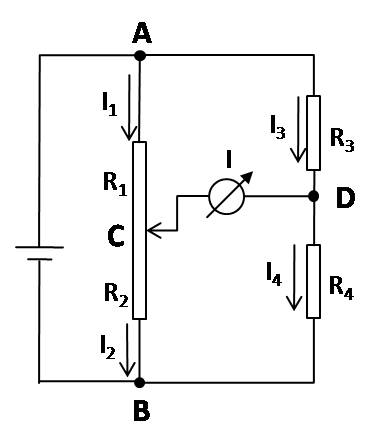
\includegraphics[width=0.7\textwidth]{Versuch_13-14/Abbildungen/Wheatstone_Prinzip.jpg}\\
 Brückenschaltung nach Wheatstone.
\end{minipage}


%------------------------------------------------
\section{Fragen zur Vorbereitung}
%------------------------------------------------

\begin{enumerate}
 %
 \item Was soll heute im Praktikum gemessen werden? Warum?
 %
 \item Wiederholung: Definition von Strom und Spannung
 %
 \item Wiederholung: Ohm'sches Gesetz, Schaltung von Messgeräten
 %
 \item Wie lauten die Kirchhoff'schen Gesetze? Welche Erhaltungssätze liegen ihnen zugrunde?
 %
 \item Wie berechnet man den Gesamtwiderstand bei Reihen- und Parallelschaltungen von Widerständen?
 %
 %\item Was ist ein Innenwiderstand?
 %
 \item Wie funktioniert die Spannungsteilerschaltung (Schaltskizze und Erklärung)?
 %
 \item Wie funktioniert die Wheatstone'sche Brückenschaltung (Schaltskizze und Erklärung)? Was kann man mit ihr messen?
\end{enumerate}

%------------------------------------------------
\section{Durchführung} 
%------------------------------------------------

\begin{minipage}{0.6\textwidth}
 \begin{enumerate}
  %
  \item Der unbekannte Widerstand $R_1$ soll mithilfe des Ohm'schen Gesetzes bestimmt werden.\\
   Erh"ohen Sie die Ausgangsspannung der regelbaren Spannungsquelle $U_1$ von 0,5\,V bis 6\,V in Schritten von 0,5\,V. Messen Sie f"ur jede Spannung den Gesamtstrom $I$ mit dem Amperemeter.\\
   Anmerkung: Ver"andern Sie w"ahrend der Messung den Widerstand $R_X$ nicht. Dann k"onnen $R_2$ und $R_x$ zum Innenwiderstand $R_i$ zusammengfasst werden, der hier nicht betrachtet werden muss.
  %
 \end{enumerate}
\end{minipage}
%
\begin{minipage}{0.35\textwidth}
 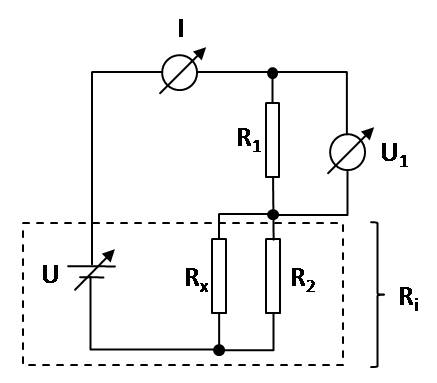
\includegraphics[width=1.00\textwidth]{Versuch_13-14/Abbildungen/Schaltung1.jpg}
 \label{fig:Schaltung1}
\end{minipage}

\begin{enumerate} \setcounter{enumi}{1}
 %
 \item Messen Sie die feste Ausgangsspannung $U_k$ mit dem Voltmeter.
 %
 \item Die drei unbekannten Widerstände $R_x$(1,2,3) sollen nach den beiden Schaltungen A und B gemessen werden. Messen Sie dazu in Schaltung A den Spannungsabfall $U_1$ am Widerstand $R_1$ und in Schaltung B den Gesamtstrom $I_1$.
 %
\end{enumerate}

%\begin{figure}[h]
\begin{minipage}[b]{0.5\textwidth}
 \centering
 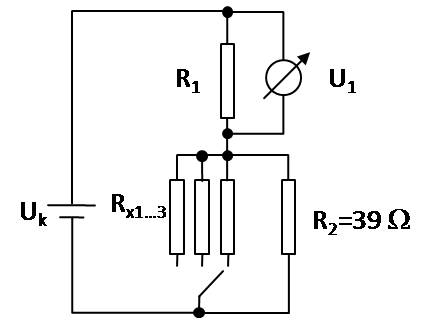
\includegraphics[width=0.7\textwidth]{Versuch_13-14/Abbildungen/SchaltungA.jpg}\\
 Schaltung A
\end{minipage}
%
\begin{minipage}[b]{0.5\textwidth}
 \centering
 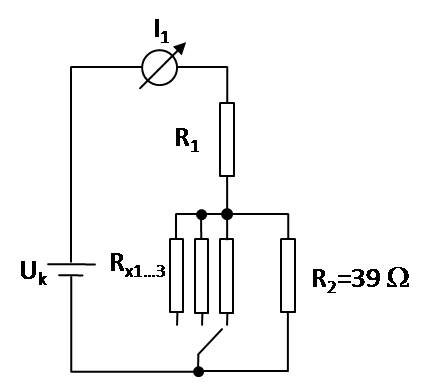
\includegraphics[width=0.7\textwidth]{Versuch_13-14/Abbildungen/SchaltungB.jpg}\\
 Schaltung B
\end{minipage}
%\end{figure}

%\begin{figure}[h]
\begin{minipage}[b]{0.6\textwidth}
\begin{enumerate} \setcounter{enumi}{3}
 %
 \item Die Innenwiderstände der Spannungsquelle und des Amperemeters sollen gemessen werden. Messen Sie dazu in Schaltung C den Gesamtstrom $I_g$ sowie die Spannung über die Lastwiderstände $U_L$. Die Größe des Widerstandes $R_3$ kann gegenüber dem großen Innenwiderstand des Voltmeters ($\approx\, 10\,M\Omega$) vernachlässigt werden. Dann berechnet sich der Innenwiderstand der Spannungsquelle nach
 \begin{equation}
  R_i = \frac{U_k - U_L}{I_g}\, .
 \end{equation}
 %
\end{enumerate}
\end{minipage}
%
\begin{minipage}[b]{0.35\textwidth}
 \centering
 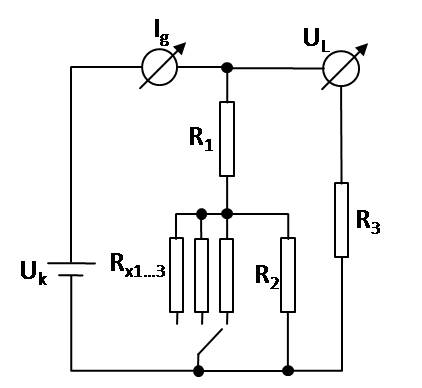
\includegraphics[width=0.8\textwidth]{Versuch_13-14/Abbildungen/SchaltungC.jpg}\\
 Schaltung C
\end{minipage}
%\end{figure}

%\begin{figure}[h]
\begin{minipage}[b]{0.6\textwidth}
\begin{enumerate} \setcounter{enumi}{4}
 %
 \item Mithilfe der Wheatstone'schen Brückenschaltung sollen die drei unbekannten Widerstände $R_y$ (y=1,2,3) bestimmt werden. \\
  Bauen sie den Versuch auf der rechten Hälfte des Experimentierschaltkreises auf. Betreiben Sie hierbei das Amperemeter im empfindlichsten Bereich.\\
  Verdrehen Sie nun das Potentiometer $R_3$ so lange, bis kein Strom mehr durch das Amperemeter fließt.\\
  Die Ablesung 'X' am Potentiometer bedeutet
  \begin{equation}
   \frac{R_{3b}}{R_{3a}} = \frac{X}{100 - X}
  \end{equation}
  und ist damit nicht direkt der Widerstand.
 %
\end{enumerate}
\end{minipage}
%
\begin{minipage}[b]{0.35\textwidth}
 \centering
 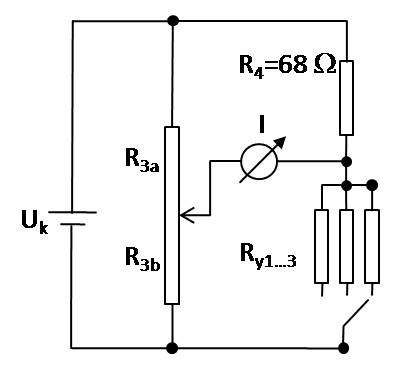
\includegraphics[width=0.8\textwidth]{Versuch_13-14/Abbildungen/Wheatstone.jpg}
 \label{fig:Wheatstone}\\
 Wheatsone'sche Brückenschaltung
\end{minipage}
%\end{figure}

%\pagebreak

%------------------------------------------------
\section{Auswertung} 
%------------------------------------------------

\begin{enumerate}
 %
 \item Berechnen Sie den Mittelwert des Widerstands $R_1$ inkl. seines Fehlers.
 %
 \item Leiten Sie die Formel für den Widerstand $R_x$ in Schaltung A her.\\
  Anleitung: Berechnen Sie den Gesamtwiderstand der Parallelschaltung von $R_x$ und $R_2$. Zusammen mit der Spannungsteilerformel erhält man schließlich:
  \begin{equation}
   R_x = R_2 \frac{1-\frac{U_k}{U_1}}{\frac{U_k}{U_1}-\frac{R_2}{R_1}-1}
  \end{equation}
 %
 \item Leiten Sie die Formel für den Widerstand $R_x$ in Schaltung B her.\\
  Anleitung: Drücken Sie $U_1$ durch den Strom $I$ aus. Danach, wie oben, einfach nach $R_x$ auflösen. Dann finden Sie:
  \begin{equation}
   R_x = R_2 \frac{R_1 - \frac{U_k}{I}}{\frac{U_k}{I}-R_1-R_2}
  \end{equation}
 %
 \item Berechnen Sie nun die Widerstände $R_x$ (x=1,2,3) aus Schaltung A und B mit ihrem Fehler. 
  Benutzen Sie eine Ungenauigkeit ($\hat{=}$ Fehler) für die Messungen der Ströme und Spannungen von 1\% .
 %
 \item Berechnen Sie den Innenwiderstand der Spannungsquelle.
 %
 \item Berechnen Sie den Widerstand $R_y$ (y=1,2,3) aus der Wheatstoneschen Brückenschaltung.\\
  Hinweis: Aus der Bedingung, dass durch das Amperemeter kein Strom fließt, ergibt sich:
  \begin{equation}
   R_y = R_4\frac{R_{3b}}{R_{3a}} \; .
  \end{equation}
\end{enumerate}